\hypertarget{de-santiago-au-duxe9sert-de-latacama}{%
\section{De Santiago au désert de
l'Atacama}\label{de-santiago-au-duxe9sert-de-latacama}}

Le Chili (continental) est une étape que nous attendions avec impatience
: on y retrouve Lisa, qui voyage depuis six mois au Brésil, et Raphaël,
qui profite de ses vacances estivales. On restera donc en famille
pendant les trois prochaines semaines, jusqu'en Colombie.

\begin{figure}
\centering
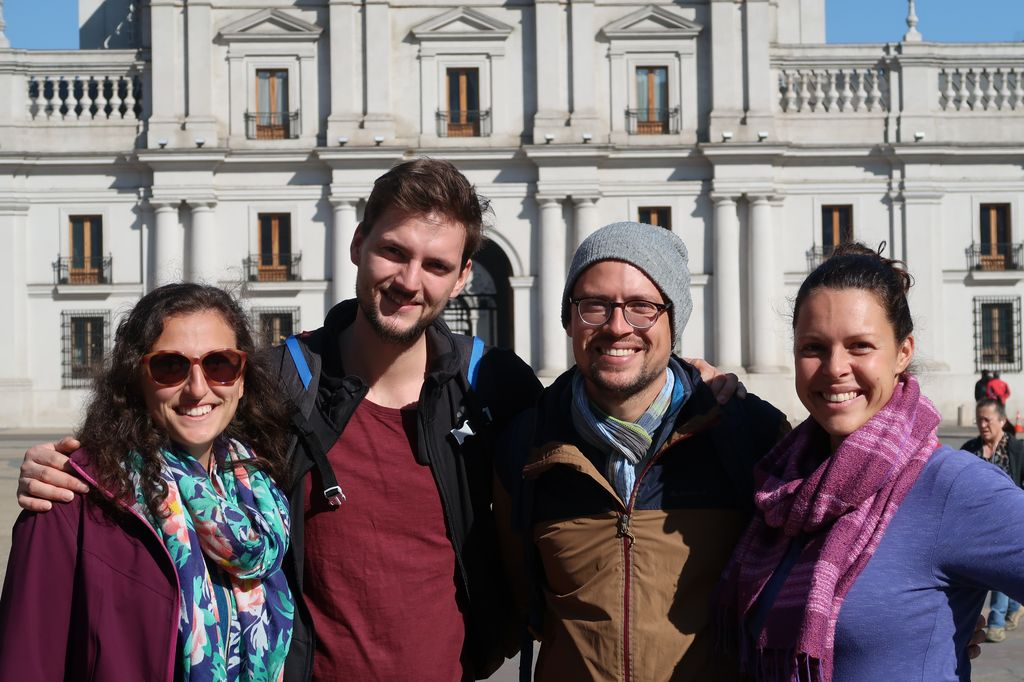
\includegraphics{images/20180904_teamsantiago.JPG}
\caption{L'équipe est au complet à Santiago !}
\end{figure}

Même si l'escale à Santiago ne durera que deux jours, nous profitons de
la situation pour faire un tour guidé à pied de Santiago ainsi que d'une
excursion à Valparaiso. A Santiago, nous faisons le plein de
connaissances sur le Chili, l'un des pays les plus développés d'Amérique
Latine (et qu'on ne connaissait pas du tout). On découvre quelques
anecdotes sur son passé récent, marqué par la dictature de Pinochet
après le coup d'état contre Allende, mais également par la domination
espagnole du temps des conquistadores (qui peinèrent à pacifier la
région des rebelles indigènes, les Mapuches).

\begin{figure}
\centering
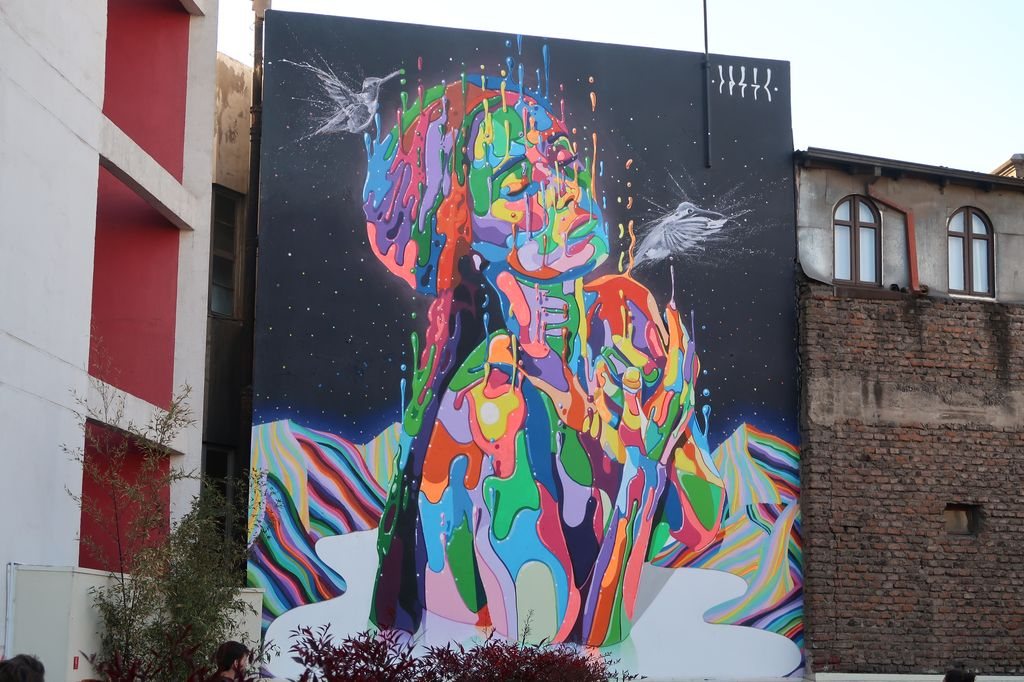
\includegraphics{images/20180904_santiagostreet.JPG}
\caption{Street art à Santiago.}
\end{figure}

Une excursion à la journée nous mène à Valparaiso, port le plus
important du Chili, connue pour ses petites rues escarpées et ses
nombreux ascenseurs. Nous y passons quelques heures dans un van conduit
par Hector, guide multilingue puisqu'il traduit ses commentaires en
espagnol, portugais et en anglais, tout au long d'un circuit entre Vina
del Mar et Valparaiso. Le tour se finit dans un quartier en hauteur où
les murs portent presque tous des fresques de street art.

\begin{figure}
\centering
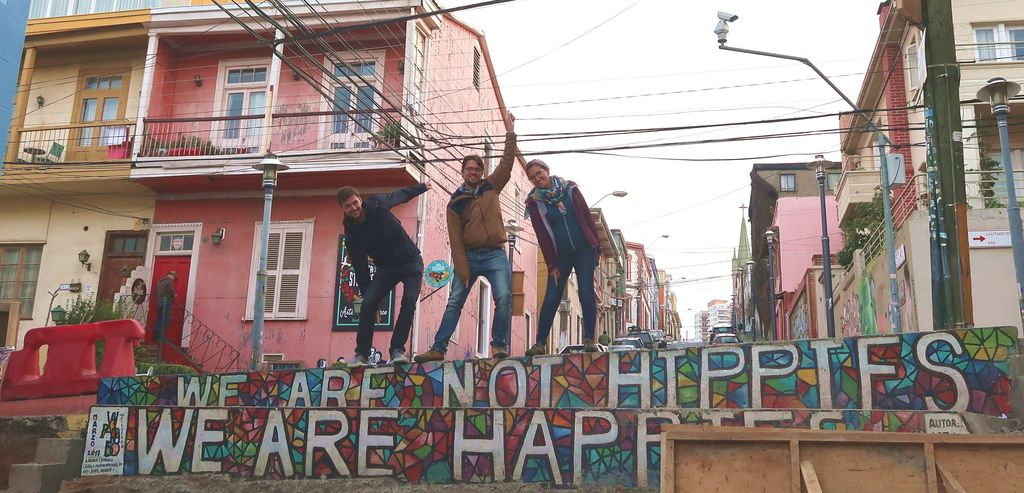
\includegraphics{images/20180904_valparaiso.JPG}
\caption{Comme le dit l'escalier en travaux "We are not hippies, we are
happies".}
\end{figure}

Nous prenons ensuite l'avion pour Calama, qui nous permet de rejoindre
San Pedro de Atacama en van. Nous sommes à ce qui restera l'un des
meilleurs moments de notre voyage. Perché sur les hauts-plateaux du
Chili, San Pedro nous permet d'accéder aux différents visages de la
terre aride de l'Atacama. C'est également la foire des tours-opérateurs
qui alpaguent les touristes fraîchement débarqués dans la rue principale
pour les convaincre de rejoindre leur bannière pendant quelques jours.
Après avoir pris quelques prix, nous sommes abordés par Marta, une
portugaise-belge en séjour indéfini à San Pedro, et prenons un "package"
avec son agence. Les prochains jours sont chargés : nous découvrons le
salar d'Atacama (version courte) et ses flamants roses,
l'impressionnante vallée de la Lune avec le coucher de soleil sur les
volcans des Andes, la lagune Cejar avec son eau glacée et très salée (où
on s'est fièrement baignés avec Raphaël), les immenses geysers du Tatio
à près de 5000 mètres d'altitude et enfin un tour quasi-privé en 4x4 en
direction du salar de Tara, à la frontière avec la Bolivie, avec pour
une fois très peu de monde autour de nous et des paysages lunaires à
perte de vue. Sans oublier un tour astronomique, lors duquel nous
découvrons un ciel si pur qu'on résiste même au froid mordant de la
nuit.

\begin{figure}
\centering
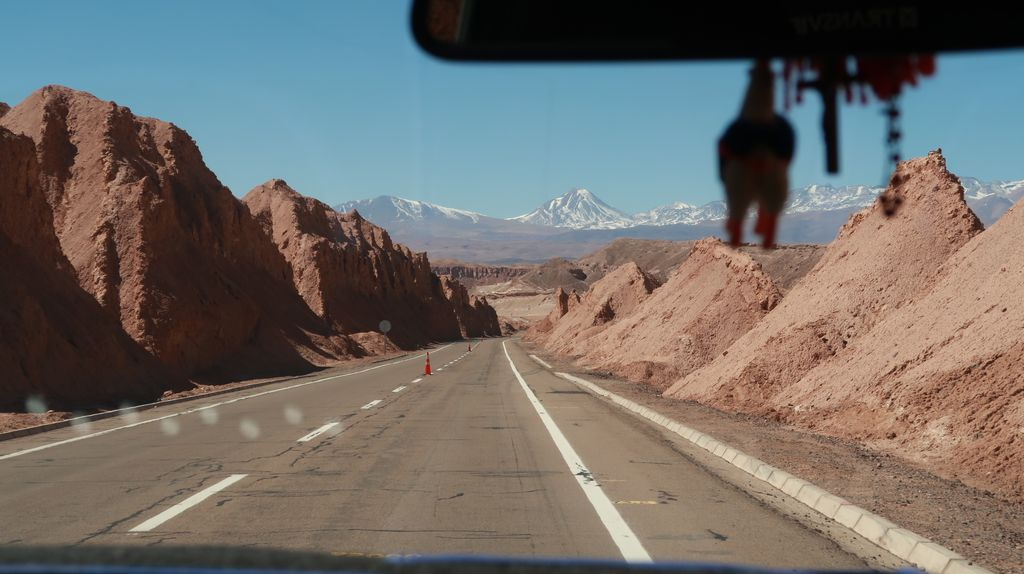
\includegraphics{images/20180904_sanpedro.JPG}
\caption{L'arrivée à San Pedro de Atacama et sa rangée de "dinosaures de
terre" à droite.}
\end{figure}

Il faut avoir vu ces paysages magnifiques ! Des reliefs du désert, des
soleils couchants et des volcans inscrits dans les traditions locales ou
encore des étoiles filantes. Nous faisons de notre mieux pour capturer
toutes ces belles choses avec notre appareil photo, comme vous allez le
voir ci-dessous. Et nous pendant ce temps-là, on vous donne rendez-vous
au Pérou !

\begin{figure}
\centering
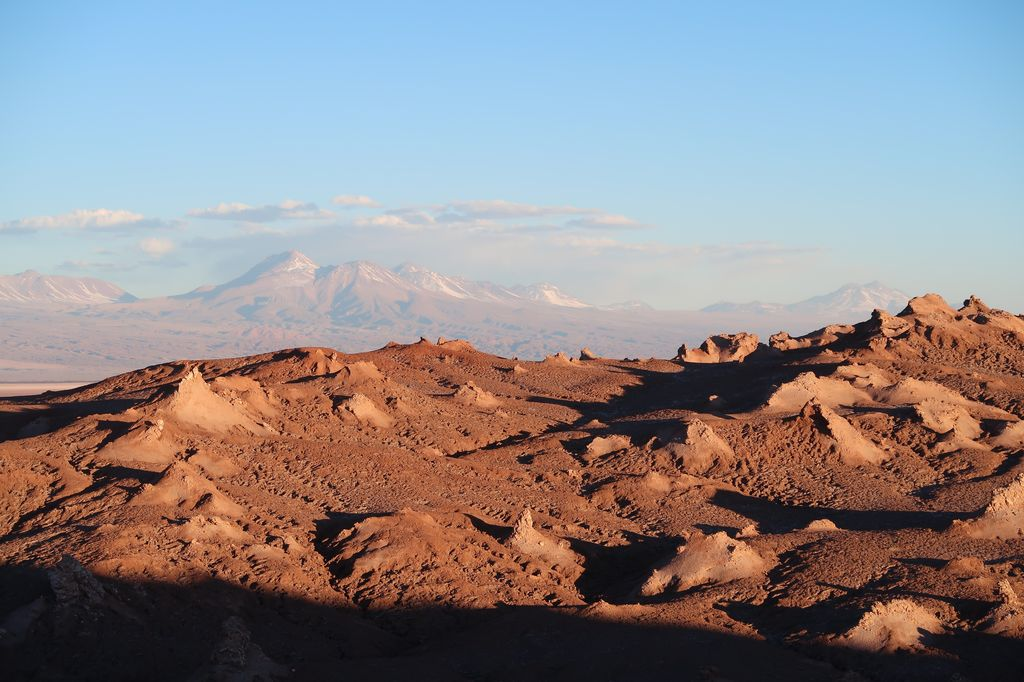
\includegraphics{images/20180904_sanpedrocoucher.JPG}
\caption{L'un des plus beaux couchers de soleil qu'on aura vu lors de
notre voyage, avec vue sur les volcans.}
\end{figure}

\emph{Florian et Elida}
